\documentclass{article}
\usepackage{amsmath, graphicx, amsfonts, caption, subfig, keyval, algorithm, algorithmic}
\captionsetup{justification=centering}
\newcommand{\R}{\mathbb{R}}
\newcommand{\C}{\mathcal{C}}
\DeclareMathOperator*{\argmin}{\arg\!\min}

\begin{document}
\title{Weighted $k$-Centers \& Lloyd's Algorithm}
\author{Jonathan Friedman \& Taylor Killiam}
\maketitle

%TODO before submission: make everything pretty and readable
\begin{abstract}
Words
\end{abstract}

\section{Introduction} \label{introduction}
Serving the maximum number of people at minimum expense is an important and general problem in industry. A company must balance placing their distribution centers near as many people as possible with the cost associated with opening and maintaining a large number of centers. In this paper, we examine a variant of the problem of placing distribution centers so that a specified cost function, such as average distance from a center, is below a given threshold. This general formulation is known as the metric $k$-center problem \cite{kmeans}. We examine the variant in which each point has a weight that affects its distance from the center point; in this case, the weight is a function of the population of the point. This leads to a metric $k$-center problem on a non-metric space. Efficient algorithms to solve this problem exist in one dimension \cite{1D}. For the two-dimensional case, we adapt Lloyd's algorithm, a clustering algorithm commonly applied to this problem, to work on this space by incorporating nonlinear least squares into the clustering step. 

If no attempt is made to avoid local extrema, then this problem is easy to solve for one center. In section \ref{onecenter}, we give a solution for one center using compass search. However, compass search is not viable for a large number of points because the number of required directions to search grows quickly. In section \ref{multicenters}, we give a solution method for an arbitrary number of centers using the modified Lloyd's algorithm. In section \ref{experiments}, we use our algorithm to optimize placement of distribution centers in Massachusetts based on population data from the U.S. 2010 Census \cite{census}, as well as to find the smallest number of distribution centers to reduce the cost function below a given tolerance level. 

% TODO: Dimensionless metric

\section{One Distribution Center} \label{onecenter}
Compass search is a simple method of minimizing a function $f \in \R^n$ that does not require computation of the gradient. The algorithm is described in Algorithm \ref{alg:compass} (see \cite{survey} for further details).

\begin{algorithm}
  \caption{Compass Sort}
  \label{alg:compass}
\begin{algorithmic}
  \STATE  Choose $\lambda_1,...,\lambda_m$ to be a positive spanning set of $\R^n$. Choose a starting guess $p_0$, a step size $s_0$, a scaling constant $\alpha<1$, and a tolerance $t$.
  \WHILE{$s_k > t$}
  \IF{$f(p_k + s_k\lambda_i) < f(p_k)$ for some $\lambda_i$}
  \STATE $p_{k+1} = p_k + s_k\lambda_i$
  \STATE $s_{k+1} = s_k$
  \ELSE
  \STATE $p_{k+1} = p_{k}$
  \STATE $s_{k+1} = \alpha s_k$
  \ENDIF
  \ENDWHILE
  \RETURN $p_{k+1}$
\end{algorithmic}
\end{algorithm}

We minimize
$$\sum_i w(\alpha_i) d(p, q_i)$$
where $p$ is the location of the point of service, $\alpha_i$ and $q_i$ are the population at and location of point $i$, $w$ is a function that weights the population, $d$ is a distance function, and the sum is over all points for which we have population data (in practice, because there are around 160,000 census blocks in Massachusetts, we subsample the population data to achieve better performance). Figure \ref{fig:popscale} shows distribution center placement for various $w$, with $d(p-q_i) = ||p - q_i||_2$. As expected, the distribution center is consistently placed near Boston. Under $w(x) = \sqrt{x}$, the center moves farther away from Boston as the influence of high population to the objective function is decreased, and under $w(x) = x^2$, the center moves closer to Boston. However, the choice of weighting function appears to have little effect on placement of the center. Even when population is not taken into account, the center remains fairly close to Boston by virtue of the large number of census blocks located there.

\begin{figure}[!ht]%
  \centering
  \subfloat[$w(\alpha_i)=\alpha_i$]{{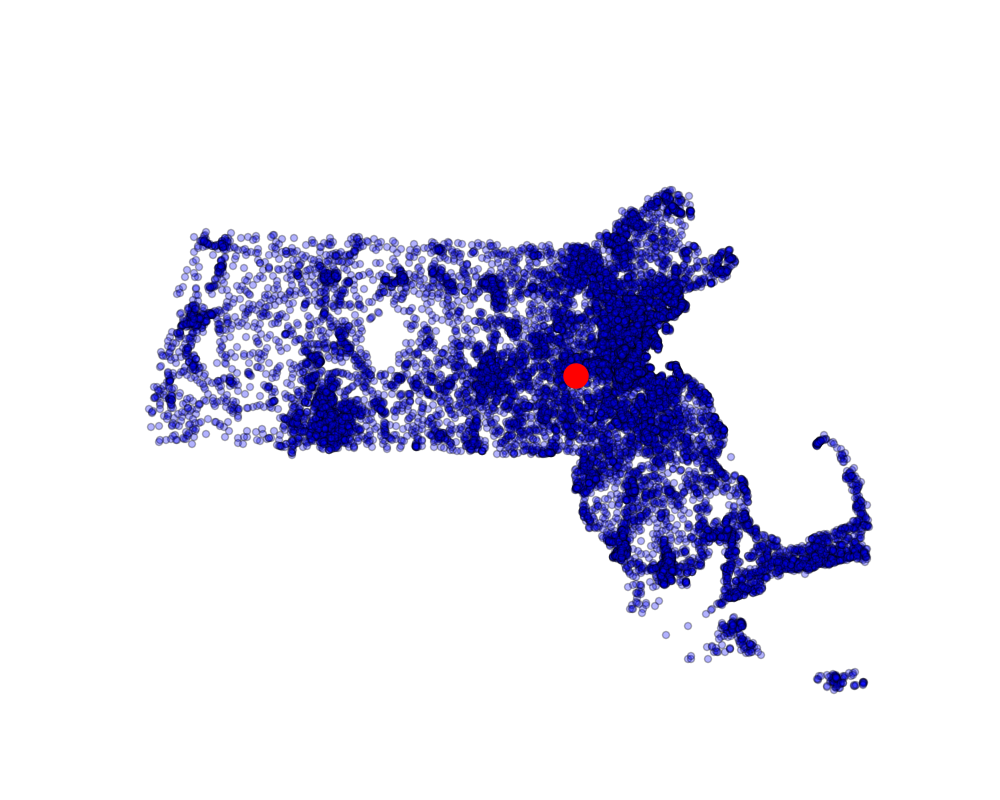
\includegraphics[width=5.5cm]{linweight.png} }}%
  \qquad
  \subfloat[$w(\alpha_i)=\sqrt{\alpha_i}$]{{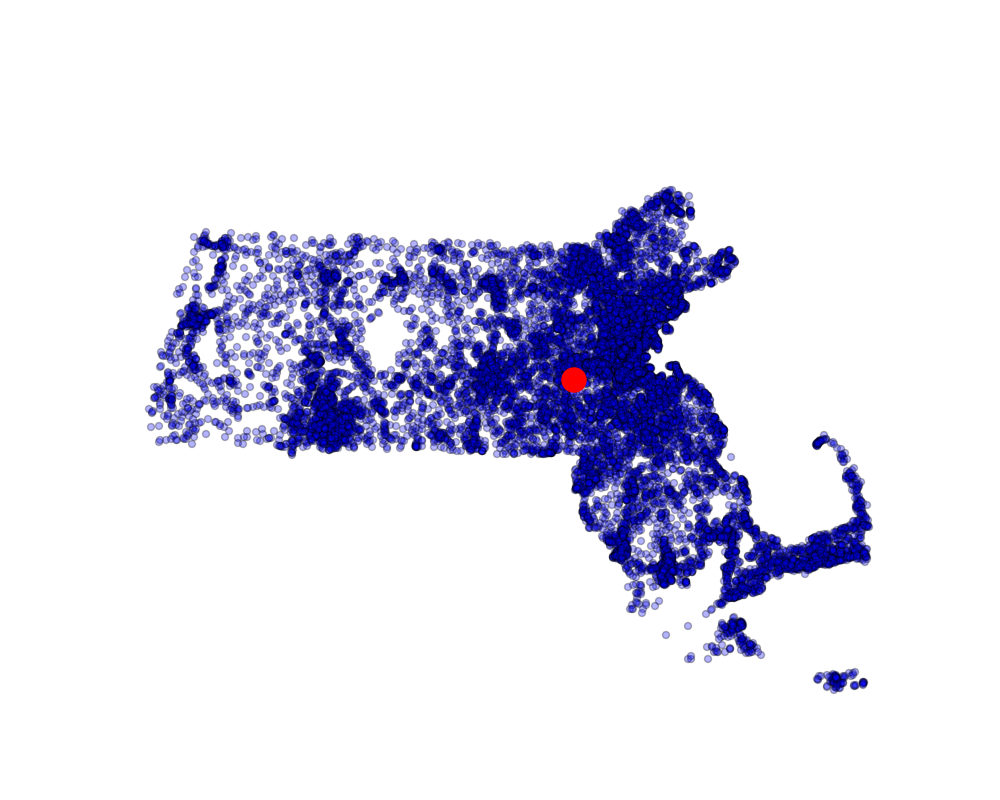
\includegraphics[width=5.5cm]{sqrtweight.png} }}%\\
  \qquad
  \subfloat[$w(\alpha_i)=\alpha_i^2$]{{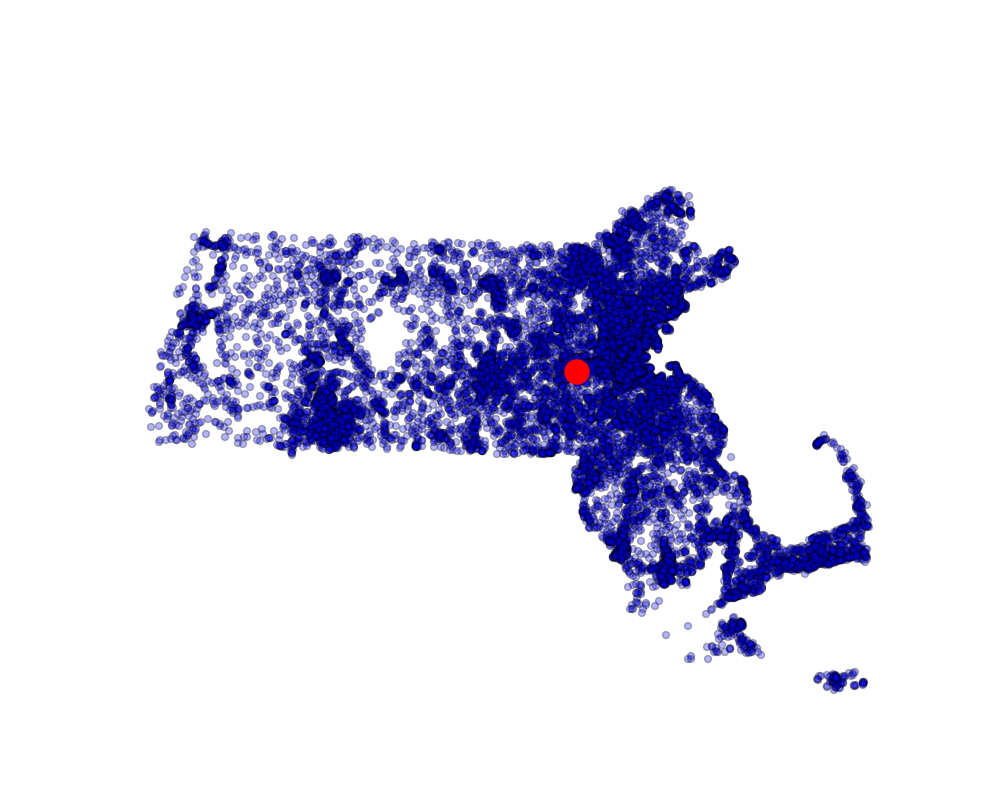
\includegraphics[width=5.5cm]{sqweight.png} }}%
  \qquad
  \subfloat[$w(\alpha_i)=1$]{{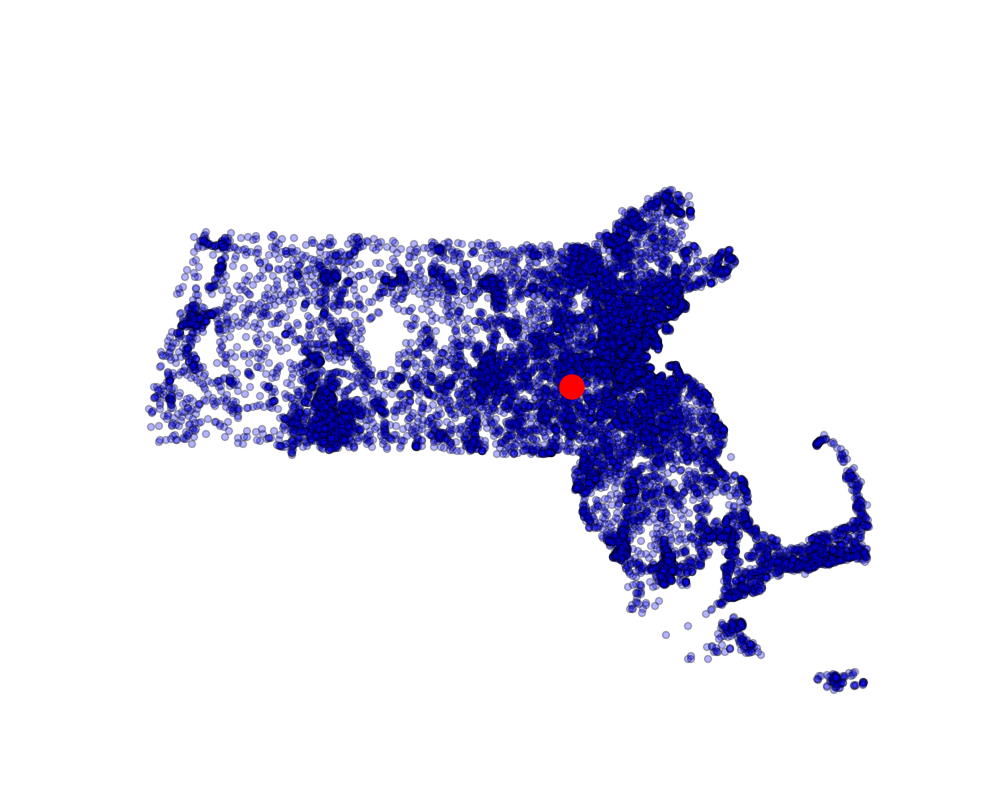
\includegraphics[width=5.5cm]{noweight.png} }}%
  \caption{Distribution center placement under various population\\scaling functions. The centers are shown in red.}
  \label{fig:popscale}
\end{figure}

This method works well for one distribution center, but the number of directions to search grows quickly with the number of centers.  Consider the case of points $c_1, ..., c_n \in \R^2$. Our function to minimize is now $$\sum_i w(\alpha_i)\min\Big(d(c_1, p_i), ..., d(c_n, p_i)\Big)$$ which corresponds to minimizing each person's distance from the nearest point of service. A positive spanning set for $\R^n$ must contain at least $n+1$ vectors \cite{charles}, so we must consider up to three possible directions at each step for each $p_i$. Determining the exact number of directions that must be searched for $n$ points in order to guarantee convergence to some maximum is beyond the scope of this paper. 

\section{Multiple Distribution Centers} \label{multicenters}
Lloyd's algorithm provides a more scaleable solution for multiple distribution centers. This algorithm was originally applied to problems in information theory \cite{lloyd}, but has been adapted to other problems, such as clustering. A detailed description is given in Algorithm \ref{alg:lloyd} (see \cite{kmeans} for further details).The general algorithm works as follows: first, assign, via some method, starting locations for the centers. Then, assign each center a cluster composed of points closer to it than to another center. Next, iteratively move the centers to the centers of their respective Voronoi cells. Repeat until the centers do not move between iterations. However, weighting points by population weights eliminates the metric structure of the space, since a point far from a center with high population, in terms of Euclidean distance, can be ``closer" than a nearby point with small population. Therefore, in the center adjusting step, we find the new location for a center $c$ in cluster $\C$ by solving the optimization problem
$$\argmin_{c} \sum_{i \in \C} w(\alpha) d(p_i, c)$$
This is equivalent to finding a root of the gradient.

A cluster is $\{p \in X : d(p, c_j) < d(p, c_k) \ \forall k \neq j\}$.

We randomly assign starting centers, though other initialization methods may be used.

\begin{algorithm}
  \caption{Lloyd's Algorithm with Nonlinear Least Squares}
  \label{alg:lloyd}
\begin{algorithmic}
  \STATE  Randomly choose $n$ centers $x_1^1, ..., x_n^1$.
  \WHILE {$\exists x_i : x_i^k \neq x_i^{k-1}$}
  \STATE Things
  \ENDWHILE
\end{algorithmic}
\end{algorithm}

This suffices to find a solution for a given number of distribution centers. To find a solution such that the cost function is below a given threshold and the number of centers is minimized, run the algorithm for $1, 2, ...$ centers until the cost function falls below the threshold. Lloyd's algorithm is not guaranteed to produce a global minimum, so to more fully explore the space, we run the algorithm several times with randomly chosen starting points for each number of centers.

\section{Experiments} \label{experiments}
\subsection{Data} \label{data}

We test our algorithms using census block population data for Massachusetts from the 2010 U.S. Census. The 2010 census divided Massachusetts into 157,508 census blocks. Population data on a block level available at \cite{census}, and can be parsed using geographic information software such as the Python Shapefile Library \cite{pyshp}. To generate a representative point for each block, we enclose the block in a rectangle, then take the center of that rectangle to be the location of the block. We generally subsampled every 50 points in order to speed up runtimes. 

%TODO: Describe we collected, parsed, subsampled, etc. census data.

\begin{thebibliography}{9}
  \bibitem{kmeans}
  Kanungo, T., Mount, D. M., Netanyahu, N. S., Piatko, C., Silverman, R., \& Wu, A. Y (2002). An Efficient $k$-Means Clustering Algorithm: Analysis and Implementation. \textit{IEEE Transactions on Pattern Analysis and Machine Intelligence 24}(7), pp. 881-892.
  \bibitem{lloyd}
  Lloyd, S. P (1982). Least Squares Quantization in PCM. \textit{IEEE Transactions on Information Theory 28}(2), pp. 129-137.
  \bibitem{census}
  U.S. Census Bureau. \textit{TIGER/Line� with Selected Demographic and Economic Data: Population \& Housing Unit Counts}. Retrieved from https://www.census.gov/geo/maps-data/data/tiger-data.html
  \bibitem{survey}
  Kolda, T. G., Lewis, R. M., \& Torczon, V (2003). Optimization by Direct Search: New Perspectives on Some Classical and Modern Methods. \textit{SIAM Review, 45}(3), pp. 385-482.
  \bibitem{charles}
  Davis, C. (1954). Theory of Positive Linear Dependence. \textit{Journal of American Mathematics, 76}(4), pp. 733-746.
  \bibitem{pyshp}
  \textit{Python Shapefile Library}. Github repository. Retrieved from https://github.com/GeospatialPython/pyshp
  \bibitem{1D}
  Chen, D. Z., Li, J., \& Wang, H. Efficient Algorithms for the One-Dimensional $k$-Center Problem (2015). \textit{Theoretical Computer Science 592}, pp. 135-142.
\end{thebibliography}
\end{document}